\section{A multidimensional taxonomy}
\label{sec:taxonomy}
\subsection{The unit is an interaction, not a label}
We define an agent as a model-driven process with a local state and an action policy, possibly including tools and repeated inference. An \emph{interacting collective} contains at least two such processes whose outputs or environmental effects can alter one another's subsequent behavior. ``Swarm'' is used as an umbrella term, without a numerical threshold or an assumption of decentralization. A population of independent samples is a relevant comparator but does not become an interacting swarm merely because its answers are later voted on.

A study may contain several collectives and several controls. We therefore code an \emph{evidence unit}: a specified system configuration, task, and comparison, rather than assigning one definitive topology to a whole paper. For example, the Opus 5.5 system card includes a five-agent peer team, asynchronous delegation, and much larger groups with task-dependent communication patterns \citep{opus55-card}. Combining them into a single row labeled ``hierarchical, 100 agents'' would erase the experiments most useful for explaining their differences.

We represent each evidence unit by
\begin{equation}
\mathcal{X}=(M,G,E,O,H,S,C,Y),
\end{equation}
where the dimensions are defined in Table~\ref{tab:taxonomy}, and Figure~\ref{fig:taxonomy} shows how they combine in one evidence unit. This is a descriptive schema, not a fitted predictive model. Fields may take multiple values. An unknown field is marked missing on that field, rather than replaced with a single uncertainty score or inferred from a product name or neighboring experiment. A report can establish the exchange medium while leaving the realized graph and token budget unknown.

\begin{table*}[t]
\centering\small
\begin{tabularx}{\textwidth}{@{}p{0.17\textwidth}YY@{}}
\toprule
Dimension & What is recorded & Distinction that prevents a false comparison\\
\midrule
$M$: model composition & Checkpoints, number of model families, roles, tools, and whether weights change & Different personas on one checkpoint versus heterogeneous models; stronger versus more diverse participants\\
$G$: interaction graph & Allowed and observed directed links; timing, recursion, routing and feedback & A designed star versus a realized hierarchy; independent candidates versus iterative exchange\\
$E$: exchange medium & Messages, files, repositories, shared context, environment, market actions, or latent vectors; whether a message is in the recipient's context when it acts & Direct chat versus influence through a common artifact or price signal; delivered versus read\\
$O$: organizational origin & Designed rules, learned policy, runtime emergence, and human interventions & Emergent roles inside a designed environment versus a policy optimized before deployment\\
$H$: memory & Private and shared stores, persistence, retrieval, provenance, update and deletion rules & Stored information versus information retrieved and correctly integrated\\
$S$: scale & Concurrent active processes, cumulative sessions or identities, and configured capacity & One coordinated team versus many unrelated tasks on the same platform\\
$C$: comparison control & Model, task, information, tools, budget, repetitions, and selection rule held fixed & Equal token cap versus equal use; best participant versus an oracle over independent runs\\
$Y$: budget and outcome & Tokens, cost, latency, accuracy, coverage, novelty, agreement, safety, and uncertainty & Time to a threshold versus final quality; consensus versus correctness\\
\bottomrule
\end{tabularx}
\caption{The proposed evidence taxonomy. Its dimensions are deliberately separate: a medium is not a graph, a graph is not its organizational origin, and an outcome is not its resource constraint. Appendix~\ref{app:evidence} applies the schema to selected evidence units.}
\label{tab:taxonomy}
\end{table*}

\begin{figure*}[t]
\centering
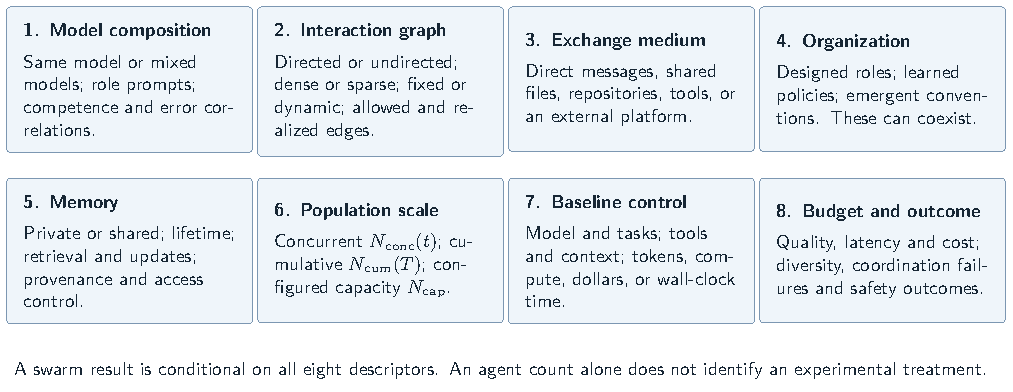
\includegraphics[width=\textwidth]{figures/taxonomy.pdf}
\caption{An evidence unit combines a system description, its comparison, and its measured consequences. Each dimension can change independently; the taxonomy records them together so a result can be transferred only with its conditions. Original diagram by the report's human--AI collaboration; no source data are plotted.}
\label{fig:taxonomy}
\end{figure*}

\subsection{Graphs, media, and organizational origin}
The communication graph should distinguish what the infrastructure permits from what agents actually do. An all-to-all chat permits dense exchange; the observed messages may concentrate around one participant. A repository allows one commit to affect many later agents without a direct message between its author and readers. The natural representation is then a temporal, bipartite graph of agents and artifacts. Reducing it to an unweighted agent graph loses both the content and the delay of influence.

The corpus contains stars, recursive hierarchies, peer exchange, sequential chains, shared workspaces, markets, and environmental coordination. These are not mutually exclusive architectures. Kimi's controller delegates to helpers that return results to it, whereas the compiler project coordinates task claims through Git files \citep{kimi-agent-swarm,anthropic-c-compiler}. Both distribute work, but a failed message and a conflicting write are different mechanisms. A market can coordinate agents that never exchange natural-language messages; a common observation can synchronize independent policies \citep{anthropic-project-swap,tokyo-road-game}.

Organizational origin adds a separate axis. \emph{Designed} organization specifies roles, routing, or scheduling outside the agents. \emph{Learned} organization optimizes these choices before a held-out task, through reinforcement learning, search, or retrospective strategy revision. \emph{Emergent} organization denotes an observed allocation of authority or labor that was not individually prescribed. These categories can coexist. Self-Organizing Agent Teams learn a frozen strategy bank before evaluation, then negotiate task-specific labor during execution \citep{sat-teams}. Agensh allows integrators to emerge at runtime inside a substantial human-designed tool and prompting environment \citep{agensh-1024}. Anthropic's 1,000-agent Fable 5.2 run supplied only one lead and 999 helpers; the lead then designed the coordination tables and reassigned helpers during the run \citep{anthropic-fable-team-scaling}. Learning can also target smaller units than an architecture. In market-based post-training (MPT), agents bid for the next turn and learn bids together with actions \citep{mpt-self-orchestration}; Waggle learns one anonymous local rule shared by interchangeable agents, so coordination forms without roles or a global topology \citep{waggle-2026}. In each case the observed structure depends on a designed environment or a learned policy.

This separation also improves the interpretation of negative evidence. Failure of a shared lock file does not refute every decentralized protocol. Success after an engineer changes the scheduler does not establish that agents discovered the scheduler. A leadership title in a prompt need not create a communication hub, as the controlled coordination study illustrates \citep{when-agents-coordinate}. We code interventions and observed behavior separately instead of resolving these differences through terminology.

\subsection{Three meanings of scale}
Let $A(t)$ be the set of active agent processes at time $t$, and let $I(t)$ be the identities or sessions observed up to that point. Then
\begin{align}
N_{\mathrm{conc}}(t)&=|A(t)|,\\
N_{\mathrm{cum}}(T)&=\left|\bigcup_{t\leq T} I(t)\right|.
\end{align}
Capacity $N_{\mathrm{cap}}$ is a configured or advertised bound; it is not an observation of either quantity. Even these definitions require a reporting convention. A process waiting on a tool may be active operationally but produce no tokens in a given interval. A restarted process may retain an identity while losing its context. Concurrency estimates therefore need their time bin, inclusion rule, and task boundary.

The enzyme campaign's 949 sessions and limit of 58 simultaneous sessions exemplify the distinction; neither implies a 949-agent concurrent team \citep{anthropic-art-enzymes}. Microsoft Research's Agensh configures 1,024 workers; in the authors' published replay, at most 1,020 identities are in a non-idle state within one displayed 37.5-second bin, our count rather than a figure the paper reports \citep{agensh-1024}. A non-idle bin does not show that 1,020 model calls ran at the same moment. The Fable 5.2 team ran 1,000 agents at once, each in its own virtual machine \citep{anthropic-fable-team-scaling}. OpenAI's report on unauthorized access counts 17,960 agents across two evaluation runs, which were not one coordinated team \citep{openai-peers-unauthorized-access}. The roughly 30,000 agents active inside Anthropic span different tasks, so the figure describes platform activity rather than a single swarm experiment \citep{anthropic-institute-pace}. Registrations add an identity problem: Moltbook advertised 1.5 million registered agents, behind which Wiz found about 17,000 human owners \citep{wiz-moltbook}, and the longest observational study counts 184,909 accounts active between 27 January and 6 October 2026 \citep{moltbook-collective-behavior}.

The frozen 3 October inventory gives a rough picture of reported population sizes. For 99 of its 153 records it holds one population size that the source reports as simultaneous within one run or one system, where the system can be an experiment, a simulated population, or a whole platform. The median of these values is seven; 42 values are at least ten, 15 at least 100, seven at least 1,000, and four at least 10,000. The field mixes meanings. Of the seven values at 1,000 or more, two come from live runs (Agensh, and a naming-game population of 1,000 agents updated one at a time), three from lab or engineering reports (Cursor's interview estimate of about 2,000, OpenAI's Navier--Stokes campaign on the order of 10,000, and about 30,000 agents working on unrelated tasks on Anthropic's internal platform), and two from surrogate populations of 10,000. None of the four values at 10,000 or more is a measured single live swarm. The statistic therefore describes how large the populations in the coded October literature were reported to be; it is not a census of concurrent teams, and we do not recompute it for later additions, whose counts appear with their meanings in Table~\ref{tab:scale}. Figure~\ref{fig:scale-chart} draws the same records by evidence class.

\begin{figure*}[t]
\centering
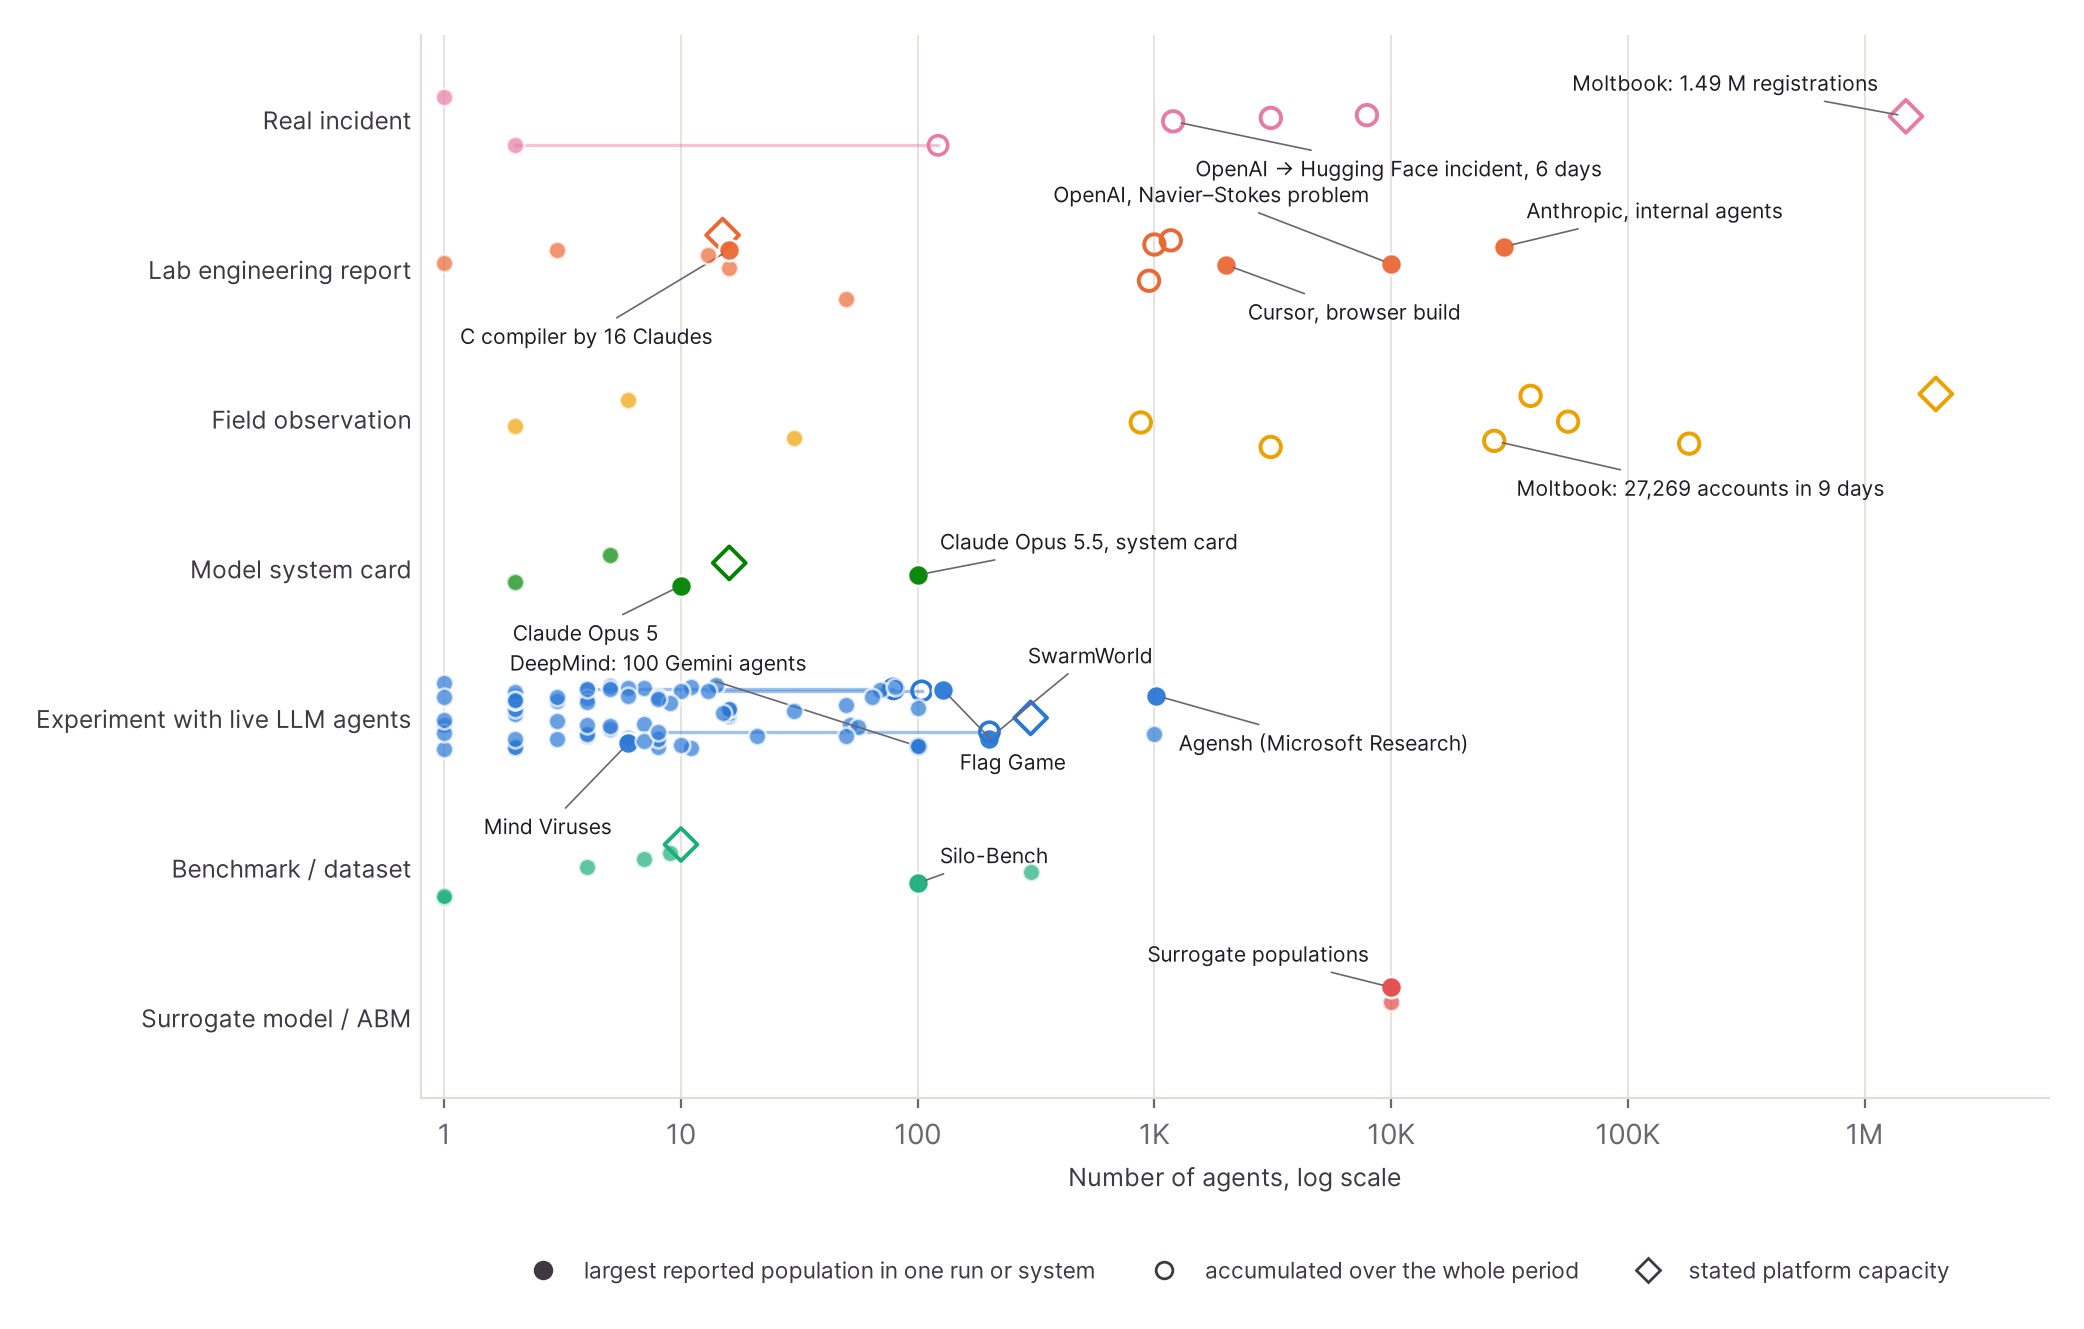
\includegraphics[width=.9\textwidth]{figures/charts/dash_scale_en_light.png}
\caption{Reported population sizes in the frozen 3 October inventory. Each point is one record, placed by the number of agents it reports (log scale) and grouped by evidence class. Filled points carry the inventory's historical class of a single reported population; that class mixes live runs, surrogate populations, and platform-wide counts across unrelated tasks, and does not establish simultaneous model inference. Open points accumulate over a whole period; diamonds are stated capacities. The largest values come from lab reports, incidents, field observations, and surrogate populations; live experiments mostly use fewer than 100 agents. Works added after 3 October are not drawn; their counts appear in Table~\ref{tab:scale}. Paper variant of the survey's chart, built from the same data by \texttt{scripts/build\_paper\_scale\_chart.py}; CC BY 4.0.}
\label{fig:scale-chart}
\end{figure*}

\begin{table*}[t]
\centering\small
\begin{tabularx}{\textwidth}{@{}p{0.25\textwidth}p{0.34\textwidth}Y@{}}
\toprule
Evidence unit & Reported count and its meaning & Population type\\
\midrule
Fable 5.2 team, Anthropic \citep{anthropic-fable-team-scaling} & 1,000 concurrent agents (one lead, 999 helpers) for 28.7 hours & Live agents; designed lead, no messaging tools\\\addlinespace[2pt]
Agensh, Microsoft Research \citep{agensh-1024} & 1,024 configured workers; at most 1,020 non-idle in one displayed 37.5-s replay bin (our count) & Live agents; staggered starts\\\addlinespace[2pt]
ExploitGym runs, OpenAI \citep{openai-peers-unauthorized-access} & 17,960 agents in two runs; 79 read peers' messages, five gained root access & Live agents, cumulative; not one team\\\addlinespace[2pt]
Moltbook, v2 \citep{moltbook-collective-behavior} & 184,909 active accounts over eight months; 1.5M registrations reported by Wiz \citep{wiz-moltbook} & Observational platform; autonomy unverified\\\addlinespace[2pt]
Network topology \citep{network-topology-consensus} & $10^3$--$10^5$ nodes on synthetic networks & Surrogate: policies extracted from four LLMs\\\addlinespace[2pt]
Inbox societies \citep{inbox-coordination-primitive} & Up to 16,000 simulated agents & Simulated society; agents with the same input share one model answer (6--23 calls per run)\\\addlinespace[2pt]
SwarmEvolve \citep{swarmevolve} & Hundreds of agents per evolutionary round & Live agents exchanging KV caches\\\addlinespace[2pt]
ScaleMAS \citep{scalemas-substrate} & Up to 128 agents on a shared substrate & Live agents\\\addlinespace[2pt]
Civ50, YC Labs and Olam Labs \citep{yc-agents-in-games} & 50 concurrent agents for three hours, about 5,900 messages & Live agents in a game world\\
\bottomrule
\end{tabularx}
\caption{Scale semantics of the largest units discussed in this edition. A concurrent team, a cumulative count across runs, a platform's account total, and a surrogate population answer different questions; none of these counts can be compared without its meaning.}
\label{tab:scale}
\end{table*}

A compact comparison with simulated robot flocks shows why these distinctions matter outside language-only tasks. COMPASS places a frozen Qwen3-1.7B model in each simulated robot and reports heading error falling from 2.79 to 0.34 degrees as the population grows from eight to 1,024 in a ``go east'' test \citep{compass-kilo-flocks}. This is a movement-control outcome in a simulated dynamical environment, not an open-ended reasoning score or a hardware deployment. Its local interaction and geometric feedback make it a useful boundary case for the taxonomy, but its population curve cannot be transferred to coding or debate accuracy.

\subsection{The baseline defines the scientific question}
A team can be compared with one ordinary invocation, one extended agent, the best individual model, a budget-matched sequential policy, an ensemble of independent runs, or a different organization. These tests answer different questions. An oracle best-of-$k$ result asks whether any independent attempt succeeds; an implemented selector asks whether the system can recognize that success. The oracle is an upper bound on selection from those candidates, not a free operational baseline. Conversely, comparing with an under-resourced single invocation can conflate coordination with additional computation.

We retain a vector of controls rather than a binary ``fair comparison'' flag. Equal tasks and tools do not imply equal information; equal token limits do not imply equal consumption; equal output tokens do not imply equal input processing or monetary cost. A mixed-model system also changes the price of a token and the capability of its components. These distinctions determine which causal interpretation is supportable, even when all authors accurately report their numbers.
